\documentclass[letterpaper,12pt]{article}

\usepackage{threeparttable}
\usepackage{geometry}
\geometry{letterpaper,tmargin=1in,bmargin=1in,lmargin=1.0in,rmargin=1.0in}
\usepackage[format=hang,font=normalsize,labelfont=bf]{caption}
\usepackage{amsmath}
\usepackage{multirow}
\usepackage{xcolor}
\usepackage{array}
\usepackage{delarray}
\usepackage{amssymb}
\usepackage{amsthm}
\usepackage{lscape}
\usepackage{natbib}
\usepackage{setspace}
\usepackage{float,color}
\usepackage[pdftex]{graphicx}
\usepackage{listings}
\lstset{basicstyle=\footnotesize\ttfamily, language=Python, showstringspaces=false}

\lstset{frame=single,
  language=Python,
  showstringspaces=false,
  columns=flexible,
  basicstyle={\small\ttfamily},
  numbers=none,
  breaklines=true,
  breakatwhitespace=true
  tabsize=3
}

\usepackage{pdfsync}
\usepackage{booktabs}
\usepackage{verbatim}
\usepackage{placeins}
\usepackage{geometry}
\usepackage{pdflscape}
\synctex=1
\usepackage{hyperref}
\hypersetup{colorlinks,linkcolor=red,urlcolor=blue,citecolor=red}
\usepackage{bm}


\theoremstyle{definition}
\newtheorem{theorem}{Theorem}
\newtheorem{acknowledgement}[theorem]{Acknowledgement}
\newtheorem{algorithm}[theorem]{Algorithm}
\newtheorem{axiom}[theorem]{Axiom}
\newtheorem{case}[theorem]{Case}
\newtheorem{claim}[theorem]{Claim}
\newtheorem{conclusion}[theorem]{Conclusion}
\newtheorem{condition}[theorem]{Condition}
\newtheorem{conjecture}[theorem]{Conjecture}
\newtheorem{corollary}[theorem]{Corollary}
\newtheorem{criterion}[theorem]{Criterion}
\newtheorem{definition}{Definition}  % Number definitions on their own
\newtheorem{derivation}{Derivation}  % Number derivations on their own
\newtheorem{example}[theorem]{Example}
\newtheorem{exercise}[theorem]{Exercise}
\newtheorem{lemma}[theorem]{Lemma}
\newtheorem{notation}[theorem]{Notation}
\newtheorem{problem}[theorem]{Problem}
\newtheorem{proposition}{Proposition}  % Number propositions on their own
\newtheorem*{proposition*}{Proposition}  % Non-numbered proposition
\newtheorem{remark}[theorem]{Remark}
\newtheorem{solution}[theorem]{Solution}
\newtheorem{summary}[theorem]{Summary}
\bibliographystyle{aer}
\newcommand\ve{\varepsilon}
%\renewcommand\theenumi{\roman{enumi}}
\newcommand\norm[1]{\left\lVert#1\right\rVert}
\newcommand{\smallsize}{\small}

\begin{document}

\hypersetup{pageanchor=false}
\begin{titlepage}
\title{The Macroeconomic Returns to Public Health Investments: Theory and Evidence from High-Burden Settings}
\date{\today}
\author{\href{http://jasondebacker.com/}{Jason DeBacker}\thanks{University of South Carolina, Darla Moore School of Business, Department of Economics, \href{mailto:jason.debacker@moore.sc.edu}{jason.debacker@moore.sc.edu}.}\and \href{https://sites.google.com/site/rickecon}{Richard W. Evans}\thanks{\href{https://abundance.institute/}{Abundance Institute}, \href{mailto:rick@abundance.institute}{rick@abundance.institute}.}\and Marcelo T. LaFleur\thanks{United Nations, \href{mailto:lafleurm@un.org}{lafleurm@un.org}.}}
\maketitle
\vspace{-2mm}
\begin{abstract}
\small{We develop a framework for quantifying the macroeconomic returns to public health investments in high-burden low- and middle-income countries. The framework combines epidemiological projections of excess mortality and morbidity with an overlapping generations general equilibrium model to recover the full dynamic path of GDP losses from health-financing contractions, and discounts those losses to a single present-value metric. Our approach can be calibrated across countries given demographic baselines, epidemiological shock paths, and treatment-financing data. We illustrate the framework using South Africa as a stress-test case---a country with high HIV/TB burden, substantial treatment coverage, and documented external financing dependence. In our preferred specification, an abrupt contraction in external health assistance implies losses exceeding 3.5\% of GDP on average over the first two decades, with net present value losses above \$1.4 trillion (2025 USD). These estimates imply benefit-to-cost ratios for external health aid that are an order of magnitude above one, underscoring that continuity of essential disease-control financing can generate large macroeconomic returns across a broad class of high-burden settings.}

\vspace{10mm}

\noindent\textit{keywords:}\: public health, external health aid, demographics, general equilibrium, overlapping generations, low- and middle-income countries

\vspace{10mm}

\noindent\textit{JEL classification:} C68, D58, E24, E37, F35, I15, J11, J17, J24


\end{abstract}
\thispagestyle{empty}
\end{titlepage}
\hypersetup{pageanchor=true}


\begin{spacing}{1.5}

\pagenumbering{arabic}

\newpage


\section{Introduction}
\label{SecIntro}

How do abrupt contractions in health financing affect long-run economic development in high-burden low- and middle-income countries (LMICs)? In many such settings, disease-control programs for HIV, tuberculosis, malaria, and other conditions are co-financed by domestic budgets and external assistance. When these flows contract, epidemiological projections imply increases in age-specific mortality and morbidity. The macroeconomic consequences of such shocks, however, depend on how they propagate through lifecycle behavior, capital accumulation, and demographic structure. In this paper, we develop a structural framework to quantify these dynamic general-equilibrium effects.

A substantial literature establishes that health conditions influence economic performance. Mortality decline increases expected lifetime income, raising savings and human capital investment in overlapping-generations (OG) settings \citep{kalemli-ozcan2000}. Epidemic mortality can weaken intergenerational human capital transmission and generate persistent income losses \citep{bell2006}. Empirically, health has been shown to enter aggregate production directly \citep{bloom2004}, and structural accounting exercises attribute a nontrivial share of cross-country income differences to health disparities \citep{Weil2007}. These contributions demonstrate that mortality and morbidity are macroeconomically consequential.

Existing work typically analyzes generic mortality decline, long-run disease burden, or cross-country health differences rather than financing-induced reversals in health outcomes. Epidemiological studies project excess deaths under funding disruptions but abstract from economy-wide feedback effects. Conversely, the aid-effectiveness literature estimates reduced-form relationships between official development assistance (ODA) and growth (e.g., \citep{BurnsideDollar:2000}), without tracing identified disease-specific financing contractions through structural demographic and capital-accumulation channels. The macroeconomic consequences of financing-induced mortality shocks therefore remain insufficiently quantified within a unified general-equilibrium framework.

We address this gap by embedding externally generated epidemiological projections into an overlapping generations (OG) general equilibrium model. Age-specific mortality shocks are constructed from projected excess deaths under alternative financing scenarios. Morbidity effects are incorporated as cohort-specific labor wedges that reduce effective labor supply. These shocks propagate through lifecycle labor supply and savings decisions, altering capital accumulation, cohort size distributions, and aggregate output. The model delivers the full transition path of macroeconomic outcomes (e.g., GDP, capital stock, employment, wages, interest rates) and microeconomic outcomes following a financing contraction relative to a no-shock baseline.

Our primary metric of economic effect is the discounted present value of cumulative GDP deviations over the transition to a new steady state. This measure aggregates intertemporal general-equilibrium effects into a single macroeconomic cost metric that is directly comparable to the fiscal cost of maintaining financing. Unlike reduced-form growth regressions or static labor-supply calculations, the framework captures capital formation, demographic feedback, and the persistence induced by cohort structure.

The model is designed to be portable across country and regional settings. All components of the model are calibrated to fit a given country or region. In our simulations of the effect of external health aid, we hold fixed the preferences, production technology, and lifecycle structure, while we exogenously change the demographic profiles, epidemiological projections, and financing exposure corresponding to our particular experiment. Given country-specific age distributions and projected mortality paths under financing scenarios, the same structural mapping can be implemented across high-burden economies. This portability facilitates cross-country comparison of macroeconomic consequences under a common structural environment.

We position the paper within three strands of literature. First, we build on OG models linking mortality to macroeconomic outcomes \citep{kalemli-ozcan2000,bell2006}, but differ by treating epidemiological counterfactuals as exogenous shock paths and focusing on transition dynamics rather than steady-state comparative statics or endogenous schooling responses. Second, we complement empirical work on health and growth \citep{bloom2004,Weil2007} by tracing dynamic general-equilibrium adjustments rather than estimating level effects or income decompositions. Third, we contribute to the literature on aid and development by providing a structural mapping from disease-specific financing contractions to long-run output losses, rather than estimating average growth responses to aggregate ODA flows.

We illustrate the framework with a South African application, where multiple independent epidemiological studies provide mortality projections under alternative financing scenarios, enabling structured sensitivity analysis within a common economic environment. The rest of the paper proceeds as follows. Section \ref{SecFramework} outlines economic model and the conceptual transmission mechanisms. Section \ref{SecData} describes the construction of mortality and morbidity shocks from epidemiological projections. Section \ref{SecCalibration} presents the model calibration and details the shock implementation. Section \ref{SecResults} reports quantitative results. Section \ref{SecDiscussion} discusses implications for financing policy in high-burden LMICs and concludes.

\section{Conceptual Framework and Empirical Setting}\label{SecFramework}


  \subsection{Model Overview}\label{SecModelOverview}

  To simulate the economy in counter-factual scenarios, we use the \texttt{OG-Core} dynamic general equilibrium model with a particular country calibration \texttt{OG-ZAF} for South Africa.\footnote{Code for the \texttt{OG-Core} open source macroeconomic model of demographic and fiscal policy is available on the GitHub platform at \href{https://github.com/PSLmodels/OG-Core}{https://github.com/PSLmodels/OG-Core}, with online documentation at \href{https://pslmodels.github.io/OG-Core}{https://pslmodels.github.io/OG-Core}. Code for the \texttt{OG-ZAF} South Africa calibration of the model is also open source and available on the GitHub platform at \href{https://github.com/EAPD-DRB/OG-ZAF/}{https://github.com/EAPD-DRB/OG-ZAF/}, with online documentation at \href{https://eapd-drb.github.io/OG-ZAF}{https://eapd-drb.github.io/OG-ZAF}. All the data and code for replicating the analyses in this paper are available in the GitHub repository \href{https://github.com/OpenSourceEcon/CostOfDisease}{https://github.com/OpenSourceEcon/CostOfDisease}.} The general \texttt{OG-Core} model and its many country calibrations feature overlapping-generations of households who vary in their labor productivity profiles. Households make choices each period about how much to work, save, and consume. These choices are made with perfect foresight, where the only uncertainty the households face is with respect to their mortality.

  In addition to households, our parameterization of the model contains a representative firm that produces output using capital and labor in a constant returns to scale production function.  The government raises revenue through individual income and payroll taxes and a corporate income tax.  This revenue is used to finance a public pension system, other transfers, government purchases of goods and service, and interest payments on any borrowing. Gaps between revenues and outlays are financed by government debt issues, although the long run of the model must have a constant debt-to-GDP ratio to ensure that no Ponzi scheme assumption is met.

  We solve the equilibrium for this model for its long-run steady state, as well as the transition path from the model's initial state to the steady state. It is this transition path that is the focus of the results presented in this paper.

  The model parameters are calibrated to match a number of characteristics of the economy one wants to simulate. These include the capital-output ratio, the debt-to-GDP ratio, the distributions of wealth and income, variations in labor productivity across the lifecycle and across skill groups, the profile of hours worked by age, average and effective marginal tax rates on households and businesses, and other salient features.  We discuss our calibration to the South African economy in more detail in Section \ref{SecCalibration}. For now, we focus on the key features of the model that are relevant for simulating improvements in health such as mortality and labor productivity.

  For complete model details, see \citet{OGCore} and \citet{DEP:2019}. Here, we present the key equations that relate the parameters of the model which are adjusted to reflect changes in labor productivity, mortality, and fertility.

    \subsection{The role of labor supply and mortality in household decisions}\label{SecLaborMort}

    The household in the model chooses savings, consumption, and labor supply in each period of life to maximize their discounted, expected lifetime utility subject to their budget constraint. The per period utility function is given as the following.\footnote{For more detail on the full theory of the household problem and references to the literature, see the online documentation for the \texttt{OG-Core} model, the chapter entitled, ``\href{https://pslmodels.github.io/OG-Core/content/theory/households.html}{Households}'' at \href{https://pslmodels.github.io/OG-Core/content/theory/households.html}{https://pslmodels.github.io/OG-Core/content/theory/households.html}.}

    \begin{equation}\label{EqHHPerUtil}
      \begin{split}
        u(c_{j,s,t},n_{j,s,t},b_{j,s+1,t+1}) &\equiv \frac{(c_{j,s,t})^{1-\sigma} - 1}{1-\sigma} + e^{g_y t(1-\sigma)}\chi^n_{s,t}\biggl(b\left[1 - \left(\frac{n_{j,s,t}}{\tilde{l}}\right)^\upsilon\right]^{\frac{1}{\upsilon}}\biggr) + \\
        &\chi^b_j \rho_{s,t} \frac{(b_{j,s+1,t+1})^{1-\sigma} - 1}{1-\sigma} \quad\forall j,t \quad\text{and}\quad E+1 \leq s \leq E+S
      \end{split}
    \end{equation}

    For a household of lifetime ability group $j$, age $s$, in time period $t$, the period utility function $u(\cdot)$ in \eqref{EqHHPerUtil} is a function of consumption $c_{j,s,t}$, labor supply $n_{j,s,t}$, and savings $b_{j,s+1,t+1}$.\footnote{We included the ``warm-glow'' bequest motive---the last term in the period utility function utility function \eqref{EqHHPerUtil}---in order to be able to more easily match the disparities in the wealth distribution we see in the data in most countries.} Note that consumption is strictly positive, while labor supply must be in the set $(0, \tilde{l}]$, where $\tilde{l}$ is the maximum fraction of a model period a household can work. The first term of the utility function is a constant relative risk aversion (CRRA) function of consumption, with a coefficient of relative risk aversion given by $\sigma$. The second term of the period utility function represents the disutility of labor supply.\footnote{This functional form approximates the common Frisch elasticity of labor supply specification. But this functional form has some convenient properties that bound labor supply to the interior of the extremes $n_{j,s,t}\in(0,\tilde{l})$. See \citet{EvansPhillips:2017}.} This disutility of labor term has a utility weight of $\chi^n_{s,t}$, which can vary by age $s$, representing changes over the lifecycle in the direct and opportunities costs of participating in market work. There is also a term in front of this component of the household utility, which is $e^{g_yt(1-\sigma)}$. This term is included so that the disutility of labor is scaled by the underlying economic growth, given by $g_y$. This scaling is necessary because household consumption and savings grow at the rate $g_y$, while labor supply is stationary. Thus, without this scaling, in the long run, the disutility of labor would shrink relative to the contributions from consumption and the bequest motive.

    The third and final term in the utility function is warm-glow bequest motive. This term has a utility weight of $\chi^b_j$, which varies by household type (i.e., skill level or productivity) in order to match the skewed distribution of bequests and wealth accumulation. Note that this term is discounted by the mortality rate, $\rho_{s,t}$, since a household only leaves a bequest if they do not survive to the next period. The function for the warm glow bequest motive is also a CRRA function with the same coefficient as the function for consumption. The functional form for the consumption and bequest motive both share the same shape. This helps ensure the model can be stationarized when there is underlying technological and population growth that increase the size of household consumption ($c_{j,s,t}$) and savings ($b_{j,s,t}$) over time.

    The household maximizes the discounted expected value of the lifetime of utility flows.
    \begin{equation}\label{EqHHmaxprob}
      \max_{\{(c_{j,s,t}),(n_{j,s,t}),(b_{j,s+1,t+1})\}_{s=E+1}^{E+S}}\: \sum_{s=1}^S\beta_j^{s-1}\left[\Pi_{u=E+1}^{E+s}(1 - \rho_{u,t+u-E})\right]u(c_{j,s,t+s-1},n_{j,s,t+s-1},b_{j,s+1,t+s}),
    \end{equation}
    where $\beta_j$ is the discount factor for households of type $j$.  Utility is maximized subject to the household's budget constraint, where the period budget constraint is given as the following:
    \begin{equation}\label{EqHHBC}
      \begin{split}
        &p_t c_{j,s,t} + \sum_{i=1}^I (1 + \tau^{c}_{i,t})p_{i,t}c_{min,i} + b_{j,s+1,t+1} = \\
        &\:\:(1 + r_{p,t})b_{j,s,t} + w_t e_{j,s,t} n_{j,s,t}  + (1-\tau^{bq}_t)bq_{j,s,t} + rm_{j,s,t} + tr_{j,s,t} + pension_{j,s,t} - tax_{j,s,t}  \\
        &\quad\:\:\forall j,t\quad\text{and}\quad E+1\leq s\leq E+S \quad\text{where}\quad b_{j,E+1,t}=0
        % p_t c_{j,s,t} + b_{j,s+1,t+1} =& (1 + r_{p,t})b_{j,s,t} + w_t e_{j,s,t} n_{j,s,t} + bq_{j,s,t} + tr_{j,s,t} + - T_{j,s,t}  \\
        % &\quad\forall j,t\quad\text{and}\quad s\geq E+1 \quad\text{where}\quad b_{j,E+1,t}=0\quad\forall j,t
      \end{split}
    \end{equation}

    The first term on the left-hand-side of the household budget constraint \eqref{EqHHBC} is total consumption expenditure, where $p_t$ is the tax-inclusive price of composite consumption by the household $c_{j,s,t}$. The second term on the left-hand-side of the budget constraint is included because we use a Stone-Geary aggregator to define the composite consumption as a function of individual consumption goods indexed by $i$.\footnote{See the section entitled, ``\href{https://pslmodels.github.io/OG-Core/content/theory/households.html\#household-consumption}{Household consumption},'' in the online \texttt{OG-Core} documentation for a full description of the household's consumption of individual consumption goods $c_{i,j,s,t}$, which are then aggregated up to a composite consumption good $c_{j,s,t}$ consumed by the household, \url{https://pslmodels.github.io/OG-Core/content/theory/households.html\#household-consumption}.}

    The first term on the right-hand-side of the household budget constraint \eqref{EqHHBC} is the return on savings from the previous period, where $b_{j,s,t}$ is the current period wealth of the household, and $r_{p,t}$ is the rate of return on the household's financial portfolio. The next term is labor income, where $w_t$ is the wage rate per effective unit of labor, $e_{j,s,t}$ is the labor productivity or effective labor of households in lifetime income group $j$, of age $s$, in period $t$. The remaining terms in the budget constraint represent income or outlays from bequests $bq_{j,s,t}$, remittances $rm_{j,s,t}$, government transfers $tr_{j,s,t}$, pension income $pension_{j,s,t}$, and net tax liability $tax_{j,s,t}$.\footnote{The online \texttt{OG-Core} documentation ``Household consumption'' section has subsections for the details on how each of these components of the budget constraint is modeled. The exception is the tax liability term $tax_{j,s,t}$, which is described in detail in the ``\href{https://pslmodels.github.io/OG-Core/content/theory/government.html\#individual-income-taxes}{Individual income taxes}'' section of the ``Government'' chapter of the online documentation, \href{https://pslmodels.github.io/OG-Core/content/theory/government.html\#individual-income-taxes}{https://pslmodels.github.io/OG-Core/content/theory/government.html\#individual-income-taxes}.}
    
    Solving the household optimization problem for the simultaneous choice of labor supply $n_{j,s,t}$, consumption $c_{j,s,t}$, and savings $b_{j,s+1,t+1}$ across a household's expected lifetime results in the following system of $S$ labor supply first-order equations \eqref{EqHHeul_n} and $S$ consumption-savings dynamic Euler equations \eqref{EqHHeul_b} and \eqref{EqHHeul_bS}, where $S$ is the maximum number of periods an individual can live.
    \begin{equation}\label{EqHHeul_n}
      \begin{split}
        &\frac{w_t e_{j,s,t}}{p_t}\bigl(1 - \tau^{mtrx}_{s,t}\bigr)(c_{j,s,t})^{-\sigma} = e^{g_y(1-\sigma)}\chi^n_{s,t}\biggl(\frac{b}{\tilde{l}}\biggr)\biggl(\frac{n_{j,s,t}}{\tilde{l}}\biggr)^{\upsilon-1}\Biggl[1 - \biggl(\frac{n_{j,s,t}}{\tilde{l}}\biggr)^\upsilon\Biggr]^{\frac{1-\upsilon}{\upsilon}} \\
        &\qquad\qquad\qquad\qquad\qquad\qquad\qquad\qquad\forall j,t, \quad\text{and}\quad E+1\leq s\leq E+S \\
      \end{split}
    \end{equation}
    
    \begin{equation}\label{EqHHeul_b}
      \begin{split}
        \frac{(c_{j,s,t})^{-\sigma}}{p_t} &= \chi^b_j\rho_{s,t}(b_{j,s+1,t+1})^{-\sigma} ... \\
        &\qquad+ \beta_j\bigl(1 - \rho_{s,t}\bigr)\left(\frac{1 + r_{p,t+1}\bigl[1 - \tau^{mtry}_{s+1,t+1}\bigr]}{p_{t+1}}\right)(c_{j,s+1,t+1})^{-\sigma} \\
        &\qquad\qquad\qquad \forall j,t, \quad\text{and}\quad E+1\leq s\leq E+S-1
      \end{split}
    \end{equation}

    \begin{equation}\label{EqHHeul_bS}
      \frac{(c_{j,E+S,t})^{-\sigma}}{p_t} = \chi^b_j(b_{j,E+S+1,t+1})^{-\sigma} \quad\forall j,t
    \end{equation}

    The optimality conditions for labor supply at each age $s$ in Equation \eqref{EqHHeul_n} equate the marginal benefit from the increased consumption from labor income with the marginal disutility of working. The marginal tax rate on labor income $\tau^{mtrx}_{s,t}$ shows up in this term, and its distortion of the labor supply decision shows up as a reduction in the marginal benefit of working.\footnote{The marginal tax rate functions $\tau^{mtrx}_{s,t}$, $\tau^{mtry}_{s,t}$ are derived from the parameterization and calibration of the broader $tax_{j,s,t}$ function found in the budget constraint \eqref{EqHHBC}. The detail for these marginal tax rate parameterizations and derivations is in the \texttt{OG-Core} online documentation ``\href{https://pslmodels.github.io/OG-Core/content/theory/government.html\#individual-income-taxes}{Individual income taxes}'' section of the ``Government'' chapter of the online documentation, \href{https://pslmodels.github.io/OG-Core/content/theory/government.html\#individual-income-taxes}{https://pslmodels.github.io/OG-Core/content/theory/government.html\#individual-income-taxes}.} We also highlight here the scale parameter on the disutility of labor $\chi^n_{s,t}$ on the right-hand-side of \eqref{EqHHeul_n}. This parameter scales the disutility of labor up and down and can vary by age $s$ and by time $t$.
    
    The consumption-savings Euler equations \eqref{EqHHeul_b} and \eqref{EqHHeul_bS} balance the marginal benefit of consumption today with the expected marginal benefit of consumption tomorrow. On the right-hand-side of the $S-1$ Euler equations \eqref{EqHHeul_b}, we see the distortionary effect of the marginal tax rates on capital income $\tau^{mtry}_{s+1,t+1}$ in reducing the marginal benefit of saving for consumption in the next period $t+1$. Equations \eqref{EqHHeul_b} also show that households discount the future through their rate of time preference, $\beta_j$, that can vary by lifetime income group, and due to mortality risk, $\rho_{s,t}$. The mortality rates $\rho_{s,t}$ vary by age $s$ and over time $t$ and are a key parameter for our mapping of the effects of public health into the macroeconomic model. As mortality rates increase, individuals discount the value of future consumption more.
    
    It is important to note that the mortality rates $\rho_{s,t}$ show up in two places in the consumption-savings Euler equations \eqref{EqHHeul_b}. As discussed in the previous paragraph, the mortality rate discounts the probability of utility from future consumption. But it also increases the probability of dying and leaving a bequest and getting utility from that bequest, as shown in the first term on the right-hand-side of \eqref{EqHHeul_b}. As the mortality rate goes down, the expected value of future consumption increases, resulting in higher savings. But a decline in mortality rates also decreases the expected value of the warm glow bequest, leading to a decrease in savings. Thus, from the household's perspective, there is an ambiguous effect of changes in mortality rates on savings and therefore in aggregate supply of capital.

    In terms of productivity, we map increases in morbidity to the disutility of labor supply $\chi^n_{s,t}$ in \eqref{EqHHPerUtil} and \eqref{EqHHeul_n}. This parameter governs the substitution effect of labor supply in that an increase in the disutility of labor supply induces a decrease in labor supply. An increase in $\chi^n_{s,t}$ will have two countervailing effects on labor supply. First, there is a direct substitution effect. Namely, if $\chi^n_{s,t}$ increases, the disutility of labor causes labor supply to decrease and households will substitute toward leisure. The countervailing effect is the income effect. As labor supply decreases, household income goes down, incentivizing the household to work more. Thus, changes in labor supply from a change in the disutility of labor have an ambiguous effect on labor supply and will depend on the relative size of the substitution versus income effects.


    \subsection{Mortality's effects on the economy}

    Moving beyond individual household choices, we consider the effects of mortality on the total population, population distribution, and aggregate economy. This is also where changes in fertility will manifest. To see this, we need to discuss, briefly, how demographics are handled in the macroeconomic model and the market clearing conditions that must be satisfied in general equilibrium.

    Let $\Omega_t\equiv\{\omega_{s,t}\}_{s=1}^S$ represent the population distribution, the number of agents of each age $s$, at time $t$. This $\Omega_t$ matrix has elements $\omega_{s,t}$, and these $\omega_{s,t}$ evolve according to the following law of motion:
    \begin{equation}\label{EqPopLawofmotion}
      \begin{split}
        \omega_{1,t+1} &= (1 - \rho_{0,t})\sum_{s=1}^{E+S} f_{s,t}\omega_{s,t} + i_{1,t}\omega_{1,t}\quad\forall t \\
        \omega_{s+1,t+1} &= (1 - \rho_{s,t})\omega_{s,t} + i_{s+1, t+1}\omega_{s+1,t}\quad\forall t\quad\text{and}\quad 1\leq s \leq E+S-1
      \end{split}
    \end{equation}

    The terms in these equations not described above are $f_{s,t}$, the fertility rates of agents of age $s$ at time $t$, and $i_{s,t}$, the rate of immigration of agents of age $s$ at time $t$. Fertility rates are given as the fraction of agents of age $s$ that have a child. Immigration rates are defined as net immigration of agents aged $s$ as a fraction of the population aged $s$. The first equation in \eqref{EqPopLawofmotion} says the number of individuals in their first period of life is equal to the number of newborns ($f_{s,t}\omega_{s,t}$) who survive infancy plus the number of net immigrants in their first period of life ($i_{1,t}\omega_{1,t}$). The second equation says the population of those older than one evolves as a function of the survival rates of those in the country plus net immigration. From these two equations we see that improvements in reproductive aging which result in increased fertility rates in turn increase the size and growth rate of the population. By contrast, decreases in mortality will increase the size of the population, but not its long-run growth rate.

    The most significant macroeconomic effects of mortality and fertility, come from their effects on the size of the population.  The market clearing conditions show this most clearly.  The market clearing condition for the labor market says that total labor demand from producers, $L_{t}$ must be equal to the total supply of effective labor units from households:
    \begin{equation}\label{EqMarkClrLab}
      L_{t} = \sum_{s=E+1}^{E+S}\sum_{j=1}^{J} \omega_{s,t}\lambda_j e_{j,s,t}n_{j,s,t} \quad \forall t
    \end{equation}

    From the labor market clearing in Equation \eqref{EqMarkClrLab}, we can see that if the population increases (through lower mortality or increased fertility), then aggregate labor supply will increase.  In equilibrium, wages will move so that this supply is met by producer demand for labor. And with higher labor demanded, more output can be produced given the aggregate production function $Y = F(K,L)$.  Note also from this market clearing condition that, holding constant labor supply, an increase in productivity ($e_{j,s,t}$) will increase the aggregate effective labor supply and increase output.

    For asset market clearing, the total demand for debt and private capital must be equal to the supply of savings from the household:
    \begin{equation}\label{EqMarkClr_Bt}
      D_{t} + K_{t} = \sum_{s=E+2}^{E+S+1}\sum_{j=1}^{J}\Bigl(\omega_{s-1,t-1}\lambda_j b_{j,s,t}\Bigr) + \text{Net Foreign Investment}_t \quad \forall t
    \end{equation}

    Lower mortality and higher fertility lead to a larger population and thus a larger supply of savings. This increase in the supply of savings will lower interest rates until the capital demanded ($K_t$) and government bonds ($D_t$) equal the supply of savings. More capital demanded by producers will increase output.


  \subsection{Conceptual Transmission Mechanisms}

  This section links epidemiological evidence to the quantitatively appropriate changes in macroeconomic model parameters. We first describe how age-specific mortality and morbidity shocks transmit to GDP in the OG framework. We then summarize why South Africa is an informative illustrative case and how that setting motivates the alternative shock paths implemented in Section \ref{SecData}. These paths ultimately generate the GDP transition dynamics and present-value GDP losses that we focus on as a summary of the economic effects of public health crises.

  Mortality shocks affect the economy through cohort size, age composition, and individual labor supply, consumption, and savings decisions. Higher age-specific mortality rates $\rho_{s,t}$ cause individuals to discount the future more and to place a higher probability on leaving a bequest. Higher mortality also reduces the number of surviving workers and changes dependency ratios, which affects labor income, household savings, and capital accumulation over time. In the model, excess mortality projections enter as changes in age-specific survival probabilities, which determine cohort size and dependency structure over time. In an intertemporal general-equilibrium setting, these demographic adjustments propagate beyond the initial health shock and shift the transition path of GDP.

  Negative morbidity shocks operate within surviving cohorts by lowering effective labor supply and labor-force participation. In the model, this channel is captured as wedges reducing effective labor supply within surviving cohorts, proxying reduced work capacity and absenteeism among exposed groups. Lower effective labor then feeds through wages, tax bases, and investment, amplifying output effects during transition.

  To isolate economic amplification, we treat the epidemiological paths as exogenous and hold the economic structure fixed across scenarios. The no-shock baseline is the model path without public health shocks, and scenario differences are interpreted as the macroeconomic effects of alternative shock magnitudes under a common structural environment. This design can be applied to any country or region by using alternative calibrations of the macroeconomic model and demographics. For a given calibration, one can simulate the shocks by changing the mortality and morbidity inputs and solve the model to find country-specific present-value output loss metrics.


  \subsection{South Africa as the Primary Illustrative Case}

  South Africa provides an informative application because it combines a high HIV/TB burden with a health system financed by both domestic resources and external health assistance. HIV prevalence remains among the highest globally, and treatment scale-up has been substantial. Estimated HIV prevalence in South African adults in 2023 ages 15 to 49 is 17.1\%, which is one of the highest rates in the world \citep{CDC2026}. In 2024, approximately 81\% of people living with HIV were receiving antiretroviral therapy and 74\% were virally suppressed \citep{unaidsdatabook2025}. The dual HIV/TB burden has measurable labor-market consequences, affecting participation, productivity, and earnings \citep{ILO2018}. These features make health shocks economically salient through both demographic structure and effective labor supply.

  External financing plays a non-trivial role in sustaining this progress. South Africa received approximately \$390 million in bilateral U.S. HIV assistance in FY2024 (PEPFAR), which represents roughly 10\% of global bilateral PEPFAR expenditures in the same fiscal year \citep{PEPFAR2024Expenditures}. In calendar year 2024, total U.S. HIV disbursements globally amounted to \$6.69 billion, including both bilateral and multilateral channels \citep{KFF2024HIVDonorFunding}. More broadly, preliminary IHME estimates indicate a sharp decline in development assistance for health in 2025, and cross-country evidence suggests that sustained reductions in external assistance could reverse recent mortality gains \citep{FGH2025,silvaImpactTwoDecades2026}. Given the scale of treatment coverage, sustained financing interruptions could disrupt service continuity for a large number of beneficiaries.

  Recent policy developments underscore this exposure. In early 2025, the US government halted health disbursements from USAID and terminated a large share of global contracts and grants \citep{Cohen2025}. For South Africa, recent epidemiological analyses project substantial excess mortality under severe withdrawal scenarios \citep{Brink2025,Gandhi2025,KS2025}. Related health-economics evidence links treatment interruptions to absenteeism and productivity losses \citep{Keogh2024,Panda2024}.

  South Africa also offers an unusual data environment for methodological calibration. Three independent epidemiological studies, each using distinct modeling frameworks, produce mortality projections for the same withdrawal scenario. This permits structured sensitivity analysis across plausible shock magnitudes under a common structural environment, making it an ideal test case for demonstrating the validity of our framework. Section \ref{SecData} constructs low, medium, and high epidemiological shock paths from these studies and maps them into model-consistent mortality and morbidity inputs for the macroeconomic simulations.


\section{Data and Scenario Construction}\label{SecData}

This section develops the general method for translating external epidemiological evidence into model-consistent shocks in an OG framework. Our approach maps the epidemiological outcomes of excess mortality and morbidity-related reductions in work capacity among surviving cohorts into our macroeconomic model inputs of age-specific mortality rates $\rho_{s,t}$ and labor-disutility scale parameters $\chi^n_s$. This method can be replicated for any country or region, given a plausible calibration of the model. We use South Africa as the primary illustrative application to demonstrate the methodology and workflow.

Our approach consists of three steps. First, we assemble one or more epidemiological shock paths from external evidence. Second, we translate excess mortality targets into age-specific mortality schedules used in the demographic block of the model. Third, we map morbidity evidence into labor-supply wedges through shifts in the labor-disutility profile. These model-consistent inputs are then passed to the OG framework to generate GDP transition paths and discounted present-value GDP losses relative to a no-shock baseline.

\subsection{Epidemiological Inputs and Scenario Design}

Let $m \in \mathcal{M}$ index alternative epidemiological scenarios. Each scenario specifies an annual excess-death target $E_m$ and a morbidity input $\Delta \chi_m$. Either component can be set to its no-shock value when evidence is available for only one channel. This structure allows the mortality and morbidity channels to be activated jointly or separately, depending on the available epidemiological inputs.

In the illustrative South Africa calibration, we draw on three independent mortality estimates under abrupt external financing contractions with limited or no domestic replacement funding. These estimates imply annual excess deaths of 81,958 \citep{Brink2025}, 132,600 (annualized from the susceptible-programming case in \citealp{Gandhi2025}), and 192,212 \citep{KS2025}. We treat these as low, medium, and high mortality targets, defining $\mathcal{M}=\{L,M,H\}$. The same procedure can be applied to alternative countries by substituting country-specific excess-death and morbidity projections.

\citet{Brink2025} use 26 country-validated Optima HIV models to project HIV-related mortality under alternative funding scenarios. We map their Scenario 5 (discontinued PEPFAR support with no mitigation) relative to Scenario 1 (status quo) for South Africa. In their Appendix Table C2, HIV-related deaths are reported as cumulative totals over 2025--2030: 251,450 under status quo and 743,200 under Scenario 5. This implies 491,750 cumulative excess HIV-related deaths over a six-year window, which annualizes to 81,958 deaths per year. Annualization is used solely to obtain a constant annual excess-death calibration target suitable for mapping into age-specific mortality rates within our macroeconomic model. We use \citet{Brink2025} as the low scenario target.

\citet{Gandhi2025} use the CEPAC-International microsimulation model to evaluate no cutbacks, partial cutbacks, and complete cutbacks in PEPFAR support over a ten-year horizon under base-case, resilient, and susceptible programming responses.\footnote{See \href{https://mpec.massgeneral.org/cepac-model}{https://mpec.massgeneral.org/cepac-model}.} In their base case, complete withdrawal increases HIV-related deaths by 601,000 over ten years relative to no cutbacks (about 60,100 excess deaths annually). In their susceptible-programming scenario, the same comparison implies 1,326,000 additional HIV-related deaths over ten years, or 132,600 annually. We use this susceptible-scenario annualized value as our medium scenario target.

\citet{KS2025} provide country-level annual lives-saved estimates by combining global cost-effectiveness parameters with country-specific U.S. aid allocations. In their Appendix Table 2, South Africa is estimated to receive 202,693 total lives saved per year from U.S. aid, of which 192,212 are attributed to HIV/AIDS. Because this is an allocation-based back-of-the-envelope estimate rather than a disease-dynamics withdrawal simulation, we interpret 192,212 as an upper-bound proxy for annual excess mortality under full withdrawal of HIV support. We use this as our high scenario target.\footnote{\citet{KS2025} note that gross HIV estimates can be upward biased by high-prevalence settings, and that country-level estimates rely on global assumptions rather than country-specific causal identification.}

Figure \ref{fig:cumDeaths} shows the cumulative excess deaths implied by these three annualized mortality targets. These excess deaths trajectories are calculated by mapping the low, medium, and high estimates described above into the mortality rates in the demographic module of our macroeconomic model and simulating the population as described in the next section.

\begin{figure}[H]
    \caption{Forecasted cumulative excess deaths in South Africa from US aid cuts}
    \label{fig:cumDeaths}
    \centering
    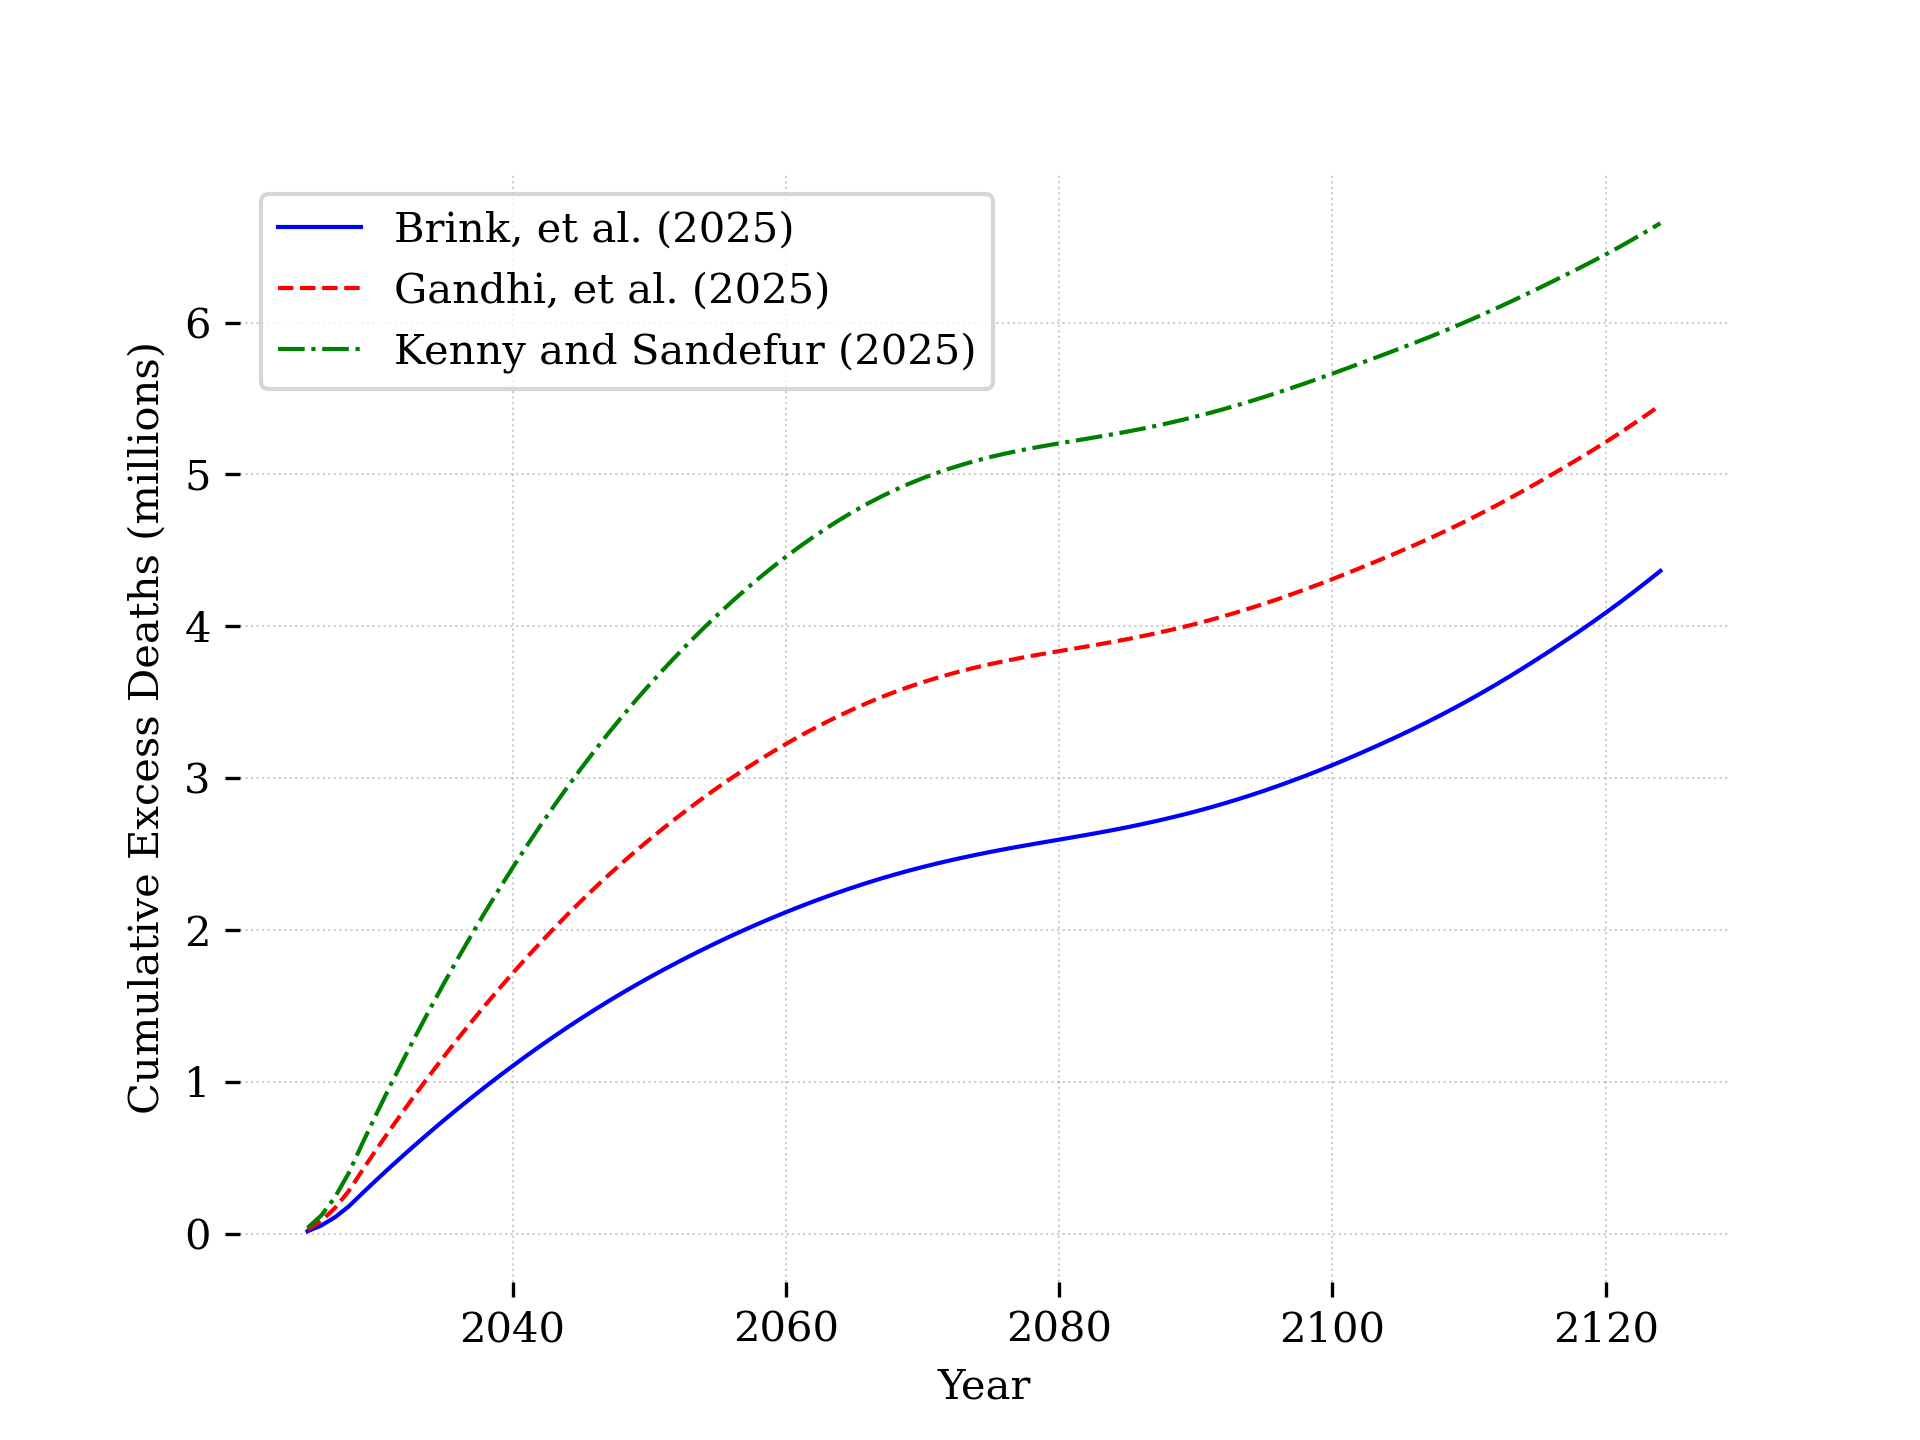
\includegraphics[scale=0.75]{./tables_figures/cumulative_excess_deaths.png}
\end{figure}

\subsection{Mapping Excess Deaths to Age-Specific Mortality Schedules}

This subsection translates scenario-level annual excess-death targets into age-specific mortality schedules used in the model's demographic inputs. Baseline mortality rates by age come from the United Nations World Population Prospects 2024 \citep{UN2024} and define the no-shock counterfactual path.

In the model, excess mortality projections enter as changes in age-specific mortality rates (equivalently, survival probabilities), which determine cohort size and age structure over time. For each mortality scenario $m$, we estimate one proportional adjustment $\varphi_m$ that scales mortality at all ages. The adjustment is chosen to match model-implied annual excess deaths in the initial full-intensity year to the target $E_m$ from Section 3.1 as closely as possible:
\begin{equation}
\varphi_m
=
\arg\min_{\varphi \ge 0}
\left[
\sum_{s=1}^{S}N_{s,0}\left(\min\{\rho_{s,0}(1+\varphi),1\}-\rho_{s,0}\right)
\;-
E_m
\right]^2
\end{equation}
where $N_{s,0}$ is baseline population at age $s$ and $\rho_{s,0}$ is baseline mortality at age $s$.

In the current implementation we apply a uniform proportional scaling across ages. This preserves the baseline age-mortality profile while increasing overall mortality to match the external annual excess-death target.

After $\varphi_m$ is identified, mortality follows a transition profile $g_t$. In the baseline implementation we use a linear five-year phase-in:
\begin{equation}
\rho_{s,t}^{(m)}=
\min\left\{\rho_{s,0}\left[1+\varphi_m g_t\right],1\right\},
\qquad
g_t=
\begin{cases}
t/5, & t=1,\ldots,5,\\
1, & t>5.
\end{cases}
\end{equation}
This implies 20\%, 40\%, 60\%, 80\%, and 100\% of the full adjustment in years 1 through 5, and full intensity thereafter. Infant mortality is held at its baseline path rather than being scaled with the mortality shock, and all mortality rates are capped at 1 by construction.

The mapping matches each annual excess-death target at full intensity. Because the shock is phased in, cumulative excess deaths over the first five years are mechanically lower than under an immediate full-shock path. The resulting age-specific mortality schedules are then passed directly to the model as scenario-specific demographic inputs. This proportional-scaling procedure can be applied to alternative demographic baselines or disease contexts by substituting country-specific excess-death targets and baseline mortality schedules. Figure \ref{fig:Mortality} shows the resulting mortality profiles for 2025.

\begin{figure}[H]
    \caption{South African mortality rates by age with and without aid}
    \label{fig:Mortality}
    \centering
    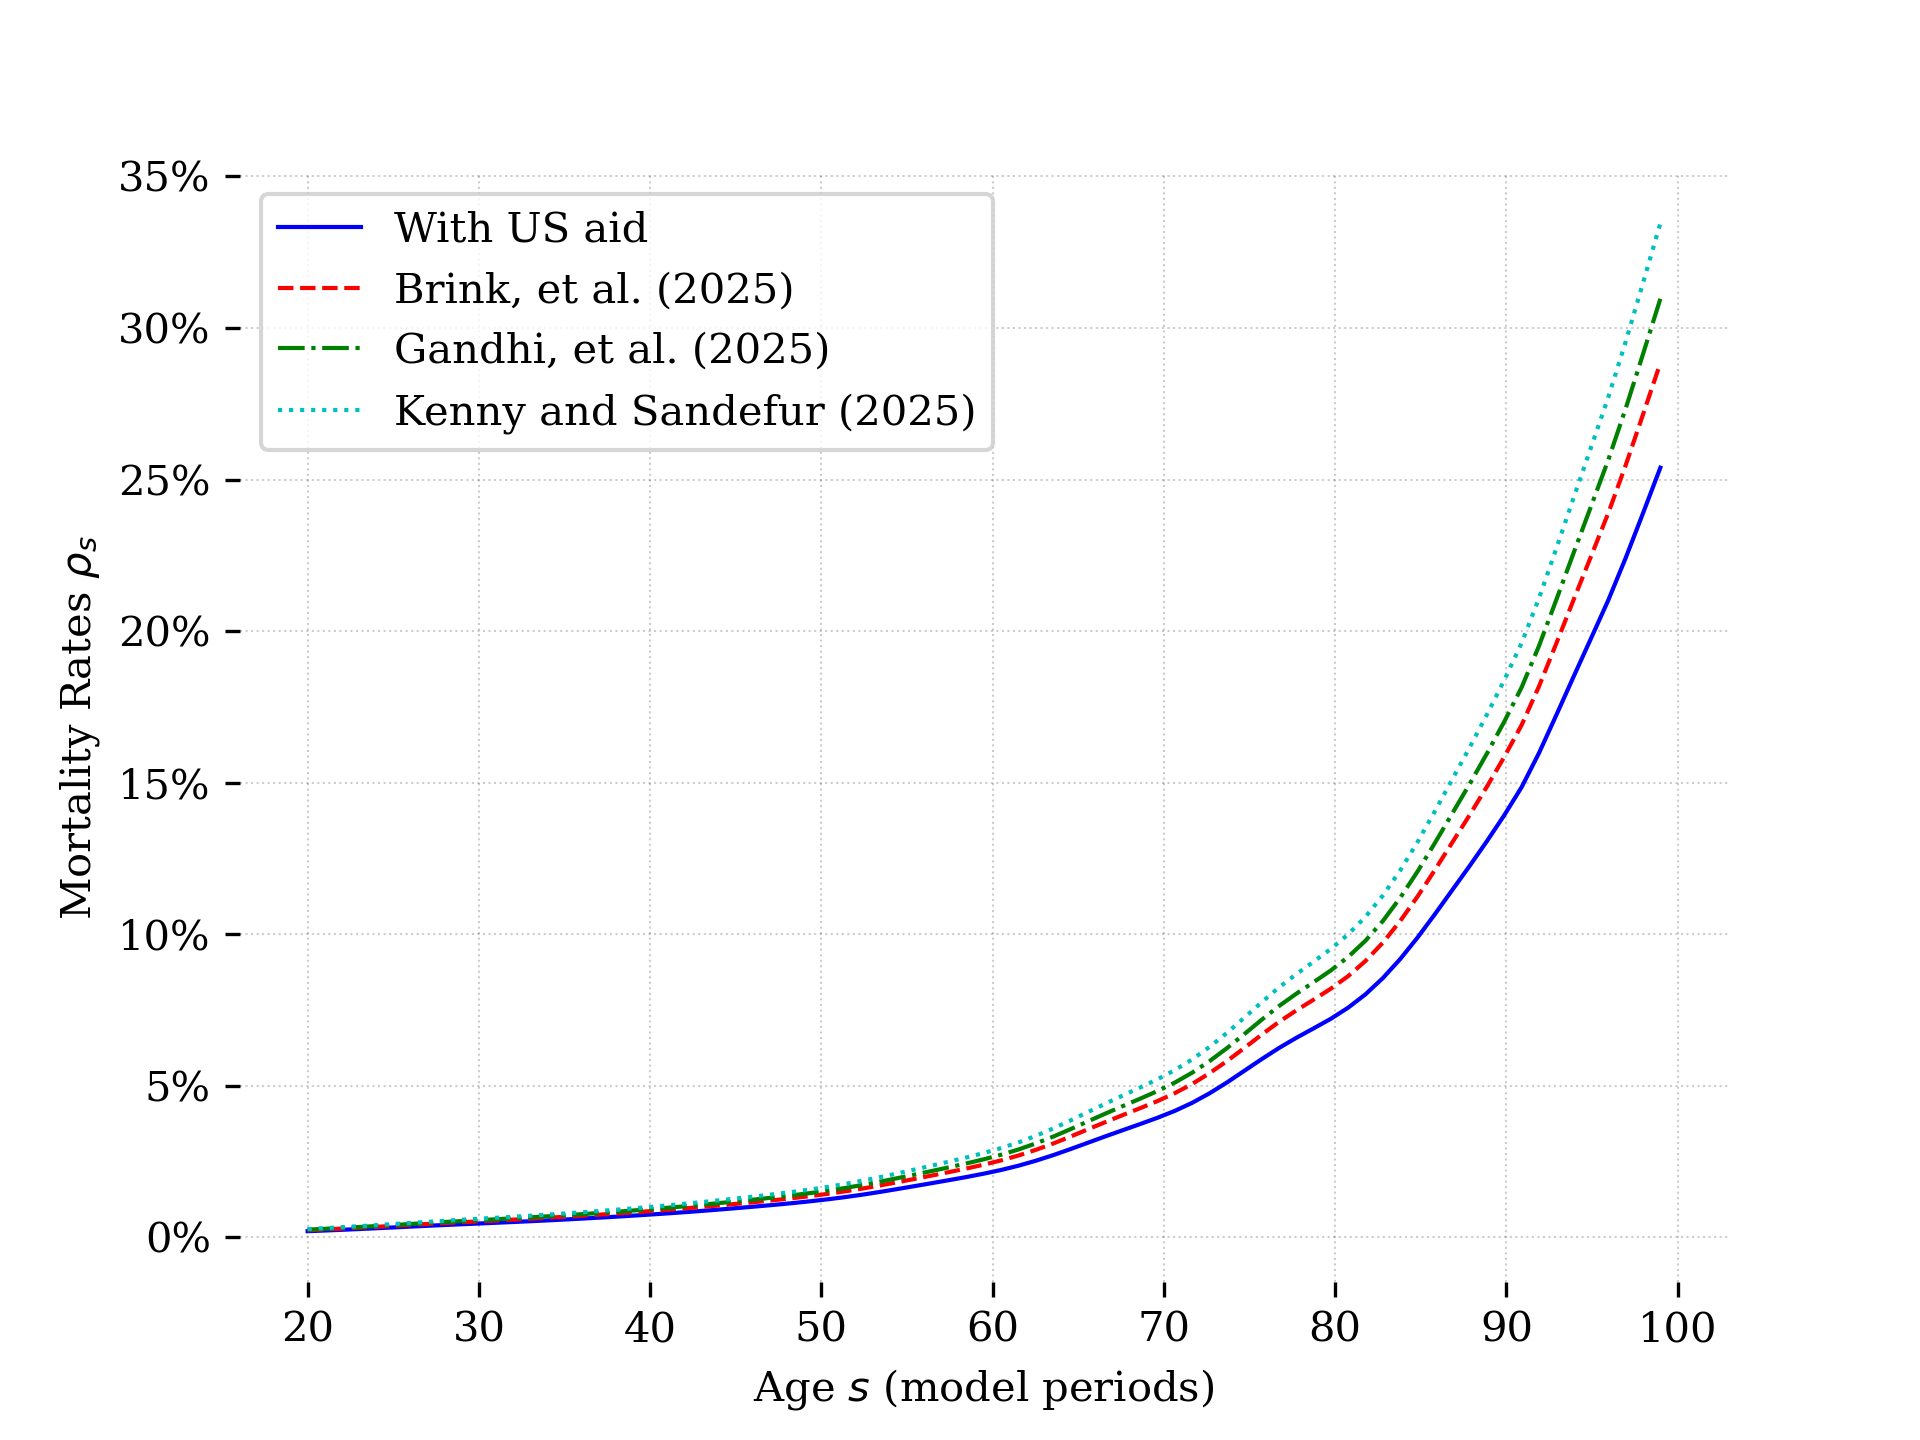
\includegraphics[scale=0.75]{./tables_figures/mortality_rates.png}
\end{figure}

\subsection{Morbidity and Labor Supply Adjustments}

To capture morbidity effects among surviving cohorts, we model treatment disruption as a reduction in work capacity that lowers effective labor supplied to the economy. In the OG setting, this channel is distinct from mortality: mortality changes cohort size and age structure, while morbidity reduces work effort and participation within surviving cohorts. We implement morbidity as a proportional increase in the labor-disutility profile, which acts as a labor-supply wedge.

The HIV component is calibrated from International Labour Office evidence on HIV-related labor-market impairment \citep{ILO2018}. The ILO framework distinguishes four channels: premature mortality, reduced productivity among employed HIV-positive workers, absenteeism and caregiving-related work losses, and turnover and retraining costs. We capture the mortality channel in Sections 3.1 and 3.2 and calibrate the morbidity wedge from the absenteeism channel. Following the ILO decomposition, absenteeism is computed as
\[
\textit{absenteeism} = (\textit{partial share} \times \textit{impairment rate}) + \textit{full share}.
\]
For South Africa, ILO series show a sharp decline in partial or full inability to work between 2005 and 2020 (from more than 163,000 people to fewer than 2,300), with corresponding absenteeism declines from about 0.52\% to 0.006\% of the working-age population (ages 15--64). This decline is consistent with expanded anti-retroviral therapy (ART) access and improved labor-market inclusion of HIV-positive individuals. We calibrate the disruption case as a reversal toward 2005 conditions. Using partial and full inability shares of 0.35\% and 0.17\%, together with the ILO high-impact impairment assumption (55\%), implies an HIV-related morbidity adjustment of 0.3606\%. This is interpreted as the incremental labor-supply penalty associated with a breakdown in treatment continuity relative to the improved ART-era baseline.

The TB component is calibrated from South Africa TB incidence profiles and work-absence effects in \citet{Keogh2024}. In that study, the high-impact specification implies a 14.4\% effect on work absences per TB case.\footnote{The underlying estimate is 17.3\%, adjusted to reflect a six-day workweek assumption in the source calculations.} We apply this high-impact effect to the total share of the working-age population (ages 15 and above) exposed to current and additional TB cases under disruption. To isolate the incremental disruption effect, we subtract baseline productivity losses computed with the low-impact case for current TB burden. This yields an additional TB-related morbidity adjustment of 0.0276\%.

The medium benchmark morbidity shock in this application is therefore
\[
\Delta\chi_{n}=0.3606\%+0.0276\%=0.3882\%,
\]
where the two terms are the HIV-related and TB-related morbidity components, respectively. In the model, morbidity enters as a proportional scaling of labor disutility:
\[
\chi^{n,m}_{s,t}=\chi^{n,0}_{s,t}\left(1+\frac{\Delta\chi_m}{100}\right).
\]
Here $\chi^{n,0}_{s,t}$ denotes the no-shock baseline labor-disutility profile and $\Delta\chi_m$ is the scenario-specific morbidity input for scenario $m$. In this application, we parameterize $\Delta\chi_m$ as
\[
\Delta\chi_m=\mathrm{mult}_{m}\Delta\chi^{n},
\qquad
\mathrm{mult}_{m}\in\{0.5,1.0,1.5\}.
\]
The index $m\in\{L,M,H\}$ denotes low, medium, and high morbidity scenarios, with $(\mathrm{mult}_L, \mathrm{mult}_M, \mathrm{mult}_H) = (0.5,1.0,1.5)$. The adjustment is imposed in 2025 and then held constant over the simulation horizon, consistent with persistent treatment disruption without full service restoration. In the current implementation, this scaling is applied uniformly to the full $\chi^n$ profile.\footnote{In OG-Core notation, $\chi^n_{s,t}$ indexes the age-specific disutility of labor in household utility, so increases in $\chi^n_s$ reduce labor supply incentives at a given wage. See Section \ref{SecLaborMort}.}

The resulting morbidity wedges are 0.194\% (low), 0.388\% (medium), and 0.582\% (high). These morbidity adjustments enter the model solely through labor-supply incentives and are analytically distinct from mortality-driven demographic effects. This mapping is also portable across settings: in other applications, researchers can replace the HIV and TB components with country-specific evidence on treatment disruption and work-capacity losses, then apply the same translation into $\chi^n$ shocks for macroeconomic simulation.


\section{Model Calibration}\label{SecCalibration}

We simulate macroeconomic effects using OG-ZAF, an overlapping generations general equilibrium model calibrated to South Africa.\footnote{OG-ZAF is an open source large scale dynamic general equilibrium overlapping generations model of the South African macroeconomy. Documentation for OG-ZAF is available at \href{https://eapd-drb.github.io/OG-ZAF}{https://eapd-drb.github.io/OG-ZAF}. Documentation for the core engine OG-Core is available at \href{https://pslmodels.github.io/OG-Core}{https://pslmodels.github.io/OG-Core}. Details of the calibration of the model are available in the ``\href{https://eapd-drb.github.io/OG-ZAF/content/calibration/households.html}{Calibration}'' section of the online documentation for OG-ZAF. The South Africa calibration includes \href{https://eapd-drb.github.io/OG-ZAF/content/calibration/households.html}{household parameters}, \href{https://eapd-drb.github.io/OG-ZAF/content/calibration/firms.html}{firm parameters}, \href{https://eapd-drb.github.io/OG-ZAF/content/calibration/macro.html}{macroeconomic parameters}, \href{https://eapd-drb.github.io/OG-ZAF/content/calibration/demographics.html}{demographics}, \href{https://eapd-drb.github.io/OG-ZAF/content/calibration/earnings.html}{lifetime earnings profiles}, \href{https://eapd-drb.github.io/OG-ZAF/content/calibration/taxes.html}{taxes}, and \href{https://eapd-drb.github.io/OG-ZAF/content/calibration/matching_lwi.html}{matching labor, wealth and income moments}.} The model includes households, firms, government taxes and transfers, and international capital flows, with age-specific demographics and labor supply decisions.  Key parameters of the calibration are summarized in Table \ref{tab:zaf_params} below.


\begin{table}[htbp]\centering\captionsetup{width=6.0in}
  \caption{\label{tab:zaf_params}\textbf{Summary of Key Parameter Values for South Africa}}
  \begin{threeparttable}
  \begin{tabular}{>{\smallsize}c |>{\smallsize}c |>{\smallsize}c}
\hline
\textbf{Symbol} & \textbf{Description} & \textbf{Value} \\
\hline
$\texttt{start\_year}$ & Initial year & 2025 \\
$J$ & Number of lifetime income groups & 7 \\
$S$ & Maximum periods in economically active individual life & 80 \\
$E$ & Number of periods of youth economically outside the model & 20 \\
$T$ & Number of periods to steady-state & 320 \\
$\beta$ & Discount factor & [0.960\ldots0.960] \\
$\sigma$ & Coefficient of constant relative risk aversion & 1.500 \\
$\nu$ & Frisch elasticity of labor supply & 0.400 \\
$b$ & Scale parameter in utility of leisure & 0.573 \\
$\chi^{b}_{j}$ & Utility of bequests level parameters & [80.000\ldots80.000] \\
$\gamma$ & Capital share of income & [0.401\ldots0.401] \\
$\varepsilon$ & Elasticity of substitution between capital and labor & [1.000\ldots1.000] \\
$\delta$ & Capital depreciation rate & 0.050 \\
$g_{y}$ & Growth rate of labor augmenting technological progress & 0.00 \\
$\alpha^{T}_{t}$ & Transfers as a share of GDP & [0.041\ldots0.041] \\
$\alpha^{G}_{t}$ & Government spending as a share of GDP & [0.267\ldots0.267] \\
$\bar{\alpha}_{D}$ & Steady-state Debt-to-GDP ratio & 1.200 \\
$\alpha_{D,0}$ & Initial period Debt-to-GDP ratio & 0.740 \\
$\tau_{d,t}$ & Scale parameter in government interest rate wedge & [0.245\ldots0.245] \\
$\mu_{d,t}$ & Shift parameter in government interest rate wedge & [$-$0.034\ldots$-$0.034] \\
$D_{f,0}$ & Share of government debt held by foreigners in initial period & 0.237 \\
$\zeta_{D,t}$ & Share of new debt issues purchased by foreigners & [0.237\ldots0.237] \\
$\zeta_{K,t}$ & Share of excess capital demand satisfied by foreigners & [0.900\ldots0.900] \\
  \end{tabular}
  \end{threeparttable}
\end{table}



This framework captures both direct and indirect channels. Direct channels include changes in survival and effective labor effort. Indirect channels include endogenous responses of capital accumulation, wages, fiscal aggregates, and relative prices. The calibration targets the demographic and macroeconomic structure of South Africa so that policy-counterfactual simulations are interpreted as deviations from a country-consistent baseline path.


\subsection{Shock Implementation and Identification of Mechanisms}\label{SecShocks}

We introduce the scenario shocks as exogenous changes to age-specific mortality and labor disutility parameters. Mortality rates transition from baseline to higher levels over 2025--2030, while the morbidity-related labor disutility wedge is imposed immediately in 2025 and then held constant. This timing reflects rapid treatment-disruption effects on absenteeism alongside more gradual cumulative mortality effects.

We treat the low, medium, and high cases as alternative externally generated epidemiological shock paths and use them as our primary sensitivity analysis. This design captures uncertainty in shock magnitude while holding the structural model and transmission mechanisms fixed, allowing transparent comparison of macroeconomic consequences across plausible mortality and morbidity trajectories.

The design enables mechanism attribution in the aggregate outcomes: mortality shocks reduce the stock of future workers, and morbidity shocks reduce effective labor supplied by surviving workers.


\section{Results}\label{SecResults}

We simulate each of the three scenarios described above with the corresponding mortality and morbidity adjustments for our South Africa calibrated macroeconomic model. The results show that the macroeconomic costs of renewed disease burden in South Africa are substantial and persistent after aid withdrawal.

The last column of Table \ref{tab:scenarios} presents the average annual GDP losses over the first 20 years of the simulation horizon. In the medium scenario, our preferred specification, South Africa's GDP declines by about \$14.8 billion per year over 2025--2044 (in 2025 US dollars), or is on average 2.1\% lower over that period than in the baseline path. Under the low excess deaths scenario, the average annual loss is about \$8.9 billion, while in the high excess deaths scenario the average annual GDP loss is about \$20.8 billion. These losses reflect persistent reductions in effective labor supply and human capital accumulation. Total global US development assistance for health was about \$21 billion in 2021, roughly the same order of magnitude as the average annual GDP loss in the high excess death scenario. If we compare the low-scenario GDP loss to U.S. health assistance to South Africa in 2023, about \$462 million, the implied annual benefit-to-cost ratio is roughly 19 to 1.\footnote{See \href{https://foreignassistance.gov}{https://foreignassistance.gov}.}

We also note that GDP impacts of disease are a potentially narrow measure of the true benefits to society of disease prevention. Therefore, our estimates should be thought of as the most conservative way to think about the costs of increased disease prevalence. However, even with this strict metric, the costs of increased disease prevalence are substantial.

\begin{table}[htbp]\centering\captionsetup{width=6.0in}
  \caption{\label{tab:scenarios}\textbf{Summary of Mortality, Absenteeism, and GDP Loss by Scenario (South Africa)}}
  \begin{threeparttable}
  \begin{tabular}{>{\smallsize}l |>{\smallsize}l |>{\smallsize}r |>{\smallsize}c ||>{\smallsize}c}
    \hline\hline
    \multicolumn{1}{c}{} & \multicolumn{1}{c}{} & \multicolumn{1}{c}{} & \multicolumn{1}{c}{} & \multicolumn{1}{c}{Avg. annual} \\
    \multicolumn{1}{c}{} & \multicolumn{1}{c}{} & \multicolumn{1}{c}{Excess} & \multicolumn{1}{c}{} & \multicolumn{1}{c}{$\Delta$ GDP} \\
    \multicolumn{1}{c}{} & \multicolumn{1}{c}{} & \multicolumn{1}{c}{deaths} & \multicolumn{1}{c}{Absenteeism} & \multicolumn{1}{c}{2026-2045} \\
    \multicolumn{1}{c}{Scenario} & \multicolumn{1}{c}{Study} & \multicolumn{1}{c}{(annual)} & \multicolumn{1}{c}{impact} & \multicolumn{1}{c}{(bil 2025 USD)} \\
    \hline\hline
    Low    & \citet{Brink2025}  &  81,958 & 0.194\% & -8.92 \\
    & & & (50\% of baseline) & \\
    \hline
    Medium & \citet{Gandhi2025} & 132,600 & 0.388\% & -14.80 \\
    & & & (baseline) & \\
    \hline
    High   & \citet{KS2025}     & 192,212 & 0.582\% & -20.82 \\
    & & & (150\% of baseline) & \\
    \hline\hline
  \end{tabular}
  \end{threeparttable}
\end{table}

Table \ref{tab:NPVLosses} summarizes the net present value (NPV) of cumulative GDP losses under each scenario, with each row representing a different discount rate used for the NPV calculation. In the medium scenario using a 2\% discount rate, the total discounted loss is about \$1.43 trillion (in 2025 US dollars). The low scenario yields a 2\% NPV loss of about \$97 billion, while the high scenario projects losses of about \$2.92 trillion. These values highlight the long-run macroeconomic consequences of disruptions to disease control and treatment services. To compare these economic costs to the cost of prevention we can take the amount of foreign assistance for health programs in South Africa before 2025 and assume this support would continue indefinitely. This assistance totaled about \$500 million per year.\footnote{See \href{https://foreignassistance.gov}{https://foreignassistance.gov}.} The NPV (at a 2\% discount rate) of providing this level of funding in perpetuity is \$25 billion. On that comparison, the medium-scenario economic losses are about 57 times larger than the cost of prevention.

\begin{table}[H] \centering \captionsetup{width=6.0in}
  \caption{\label{tab:NPVLosses}Net Present Value of GDP Loss (billions of 2025 USD), South Africa}
  \begin{tabular}{lrrr}
    \hline\hline
    Discount & Low scenario & Medium scenario & High scenario \\[-1.5mm]
    rate & \citet{Brink2025} & \citet{Gandhi2025} & \citet{KS2025} \\
    \hline\hline
    1\% & 366.87 & -2,170.78 & -5,017.86 \\
    2\% & -97.10 & -1,429.06 & -2,917.81 \\
    3\% & -230.87 & -979.36 & -1,811.41 \\
    4\% & -245.24 & -696.57 & -1,194.65 \\
    6\% & -188.00 & -388.01 & -604.48 \\
    \hline\hline
  \end{tabular}
\end{table}

These results indicate that the economic burden of disease extends far beyond the direct costs to the health sector. Even in the more optimistic scenario, where the health system absorbs much of the shock, the loss in output is substantial. The high-impact scenario shows that a collapse in treatment access and mitigation capacity could result in losses equivalent to 5.5\% of South Africa's 2023 GDP.\footnote{South Africa's GDP in 2023 was \$380 billion.}

The spread in outcomes across low, medium, and high scenarios should be interpreted as sensitivity to epidemiological input uncertainty rather than full parametric uncertainty of all model assumptions. Even under this conservative framing, the implied long-run macroeconomic losses remain large and persistent. These South Africa results are best understood as one realization of the framework under a particular demographic structure, disease profile, and external financing composition. 

\section{Discussion and Policy Implications}\label{SecDiscussion}

This paper develops and illustrates a portable framework for quantifying the macroeconomic returns to external health aid in high-burden low- and middle-income countries. The framework combines epidemiological mortality projections and morbidity-based labor shocks within a calibrated overlapping generations general equilibrium model, and summarizes the results as a discounted present-value GDP loss that is directly comparable to the cost of maintaining the financing.

Applied to South Africa as a primary illustration, our preferred medium scenario implies average GDP losses of about 3.5\% over the first two decades and discounted losses of about \$1.43 trillion at a 2\% discount rate, against an NPV cost of aid in perpetuity of roughly \$25 billion. The implied benefit-to-cost ratio of about 57:1 is illustrative of the potential macroeconomic returns across a broad class of high-burden settings.

The central methodological contribution is a transparent mapping from epidemiological evidence to general-equilibrium output dynamics that can be specifically calibrated across countries. Health-financing disruptions create persistent macroeconomic damage through interacting mortality and labor channels, and the magnitude of these effects depends systematically on demographic structure, disease burden, and external financing composition.

Our results underscore the fragility of growth in settings of high disease burden and where treatment access hinges on foreign aid. They also highlight the risks of short-term budget decisions with long-term developmental consequences. Macroeconomic modeling of public health investments allows a quantitative assessment of the short-, medium-, and long-run costs and benefits of these investments.

A key feature of the framework is its portability across the broader class of high-burden LMICs that depend on external health financing. The OG-Core ecosystem includes country-calibrated OG models for multiple high-burden settings, which lowers the marginal cost of adapting this analysis to new countries. Our South Africa application illustrates the range of the framework under well-documented epidemiological projections.

To extend the policy takeaways beyond the analyses in this paper, it is useful to consider what drives cross-country variation in the implied macroeconomic losses. The framework suggests three primary factors. First, disease burden and treatment coverage are critical as countries with higher disease prevalence and more treatment-dependent populations are exposed to larger morbidity and mortality shocks under financing disruptions. Second, demographic structure has large effects as countries with younger age profiles and higher shares of working-age population experience larger labor-supply effects from mortality because more of the shock falls on productive cohorts. Third, external financing composition matters. Countries where external aid represents a larger share of total disease-control expenditure face steeper coverage reductions under equivalent financing shocks. These three dimensions jointly determine the macroeconomic sensitivity of a country to external health-financing volatility and can be used to rank exposure across the broader population of aid-dependent high-burden settings.

To guide implementation in other settings, applications require four core country inputs: baseline demographic schedules by age, epidemiological shock paths for mortality and morbidity, labor-market exposure parameters that map morbidity into effective labor supply, and treatment-financing composition including expected domestic mitigation under aid shocks. Given these inputs, the same structural mapping can be re-calibrated to generate country-specific transition paths for output and other welfare-relevant aggregates.

Some assumptions in the baseline specification are context-sensitive and may not transport one-for-one. In particular, the mapping from aggregate excess deaths to age-specific mortality schedules, the proportional scaling of morbidity wedges across scenarios, and the incidence of morbidity effects across skill groups should be re-estimated when local evidence is available. A practical extension roadmap is to prioritize three robustness margins in new applications: alternative age-mortality mappings, explicit mitigation scenarios with partial domestic replacement, and alternative exposure incidence across skill and informal-sector groups.

More broadly, the large benefit-to-cost ratios estimated here---about 57:1 on an NPV basis in the South Africa medium scenario---are consistent with the broader development literature showing high returns to public health investments in LMICs \citep{coleImpactPoorHealth2006,turanLifeExpectancyEconomic2020}. They suggest that external health assistance to high-burden countries is not merely humanitarian in character but generates substantial macroeconomic returns. This reframing has practical implications: public health organizations and development finance institutions should assess the potential economic returns from health aid, negotiate methods for delivery of services, and innovate methods to finance these expenditures, particularly for countries that lack the financial capacity and expertise to build and maintain the necessary public health infrastructure independently.

Given our estimated high returns to public health investment and the likelihood that most of the benefits accrue within the country, another implication is that these are some of the best internal investments of public funds. Many LMICs are cash constrained, and the desired public health services often require humanitarian and organizational expertise that is not present in the country. But subsidized loans to LMICs to facilitate public health investment is likely an important addition to foreign direct investment in the portfolio of public health options.

The structural approach of this paper also complements the empirical aid-effectiveness literature, which has documented significant heterogeneity in reduced-form aid-growth relationships \citep{BurnsideDollar:2000}. Our framework suggests that one dimension of this heterogeneity is disease-specific: financing disruptions in high-burden settings operate through identifiable demographic and labor-supply channels that amplify the macroeconomic cost well beyond the immediate budgetary value of the aid withdrawn. Integrating structural estimates of these channels into cost-benefit analyses of aid allocation could improve the targeting of health assistance toward the settings with the highest macroeconomic returns.


\end{spacing}

\section*{Data availability}

All Python code and documentation for the computational examples and analyses are available at \href{https://github.com/OpenSourceEcon/CostOfDisease}{https://github.com/OpenSourceEcon/CostOfDisease}.


\bibliography{CostOfDisease.bib}


\end{document}
